\chapter{Theory}
%Necessary theoretical background

\section{Thermodynamic Limit}
In the thermodynamic limit,
\begin{equation}
	N\rightarrow\infty, V\rightarrow\infty, \frac{N}{V} = const.
\end{equation}

As stated earlier in computer simulations the concept of $\infty$ is completely redundant.
Computers retain a restricted amount of memory available to perform calculations.
To this end, simulations in general study the behaviour of smaller systems.
Depending on the complexity of the problems invovled and how co-related each site is, you often find a large range in sizes from $8x8$ up to several thousand.
Assuming momentarilly you could perform computer simulations for an inifinite lattice, you would find results that after reasonable thermalisation and statistical analysis that are identical to a theoretical prediction.
As stated earlier, the number of lattice sites you can reasonablly use for simulation purposes is restricted.
This introduces boundary effects and noise that are not present on an inifite grid.
To reduce this problem you turn to your lattice construction.

\section{Lattice}
As stated earlier, it is impossible to perform computer simulations for inifite lattice sizes.
By shrinking the lattices down to useable sizes you typically introduce boundary effects that can add a layer of noise to the data.
To reduce the effects of boundary noise, you can enforce periodic boundary conditions on your lattice such that
\begin{equation}
	\begin{split}
		s_{i=L,j=0} = s_{i=0,j=0}  \\
		s_{i=0,j=L} = s_{i=0,j=0}
	\end{split}
\end{equation}
In a physical sense taking a 2 dimensional lattice and enforcing such boundary conditions upon it leads to a torus as shown below.
\begin{figure}[h!]
	\centering
	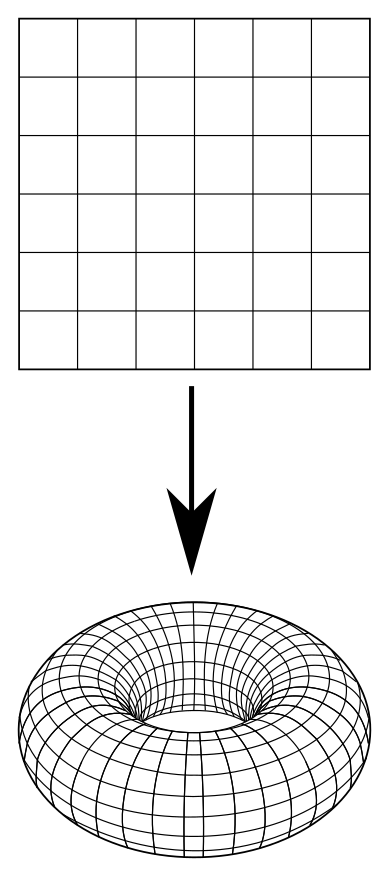
\includegraphics[width=0.25\textwidth]{2-Theory/latticetotorus.png}
	\caption{2 dimensional lattice transforming to torus under periodic boundary conditions}
\end{figure}

\section{Interfaces}

\section{Observables}
	\subsection{Magnetisation}
	Materials are often classified by their responses to externally applied fields.
	The types of response to the applied fields are diamagnetic, paramagnetic or ferromagnetic.
	Diamagnetism is the weakest response and opposes the applied magnetic field.
	Paramagnetism is stronger than diamagnetism and is proportional to the field strength and aligned to the direction.
	Ferromagnetism, is the type of magnetism studied in this project, the effects of this type of response can occasionally be orders of magntitude larger than of the other types.
	In this project, we have no externally applied field.
	Diamagnetism and Paramagnetism in this case do not apply because they are in response to an externally applied field.
	\begin{equation}
		M=\sum_{i}^{V}\sigma_{i}
	\end{equation}

	\subsection{Energy}
	\begin{equation}
		H=E=-\sum_{i,j}\delta (\sigma_i,\sigma_j)
	\end{equation}

	\subsection{Specific Heat}
	\begin{equation}
		C=\beta^2[<E^2>-<E>^2]
	\end{equation}

	\subsection{Magnetic Susceptibility}
	\begin{equation}
		\chi=\beta[<M^2>-<M>^2]
	\end{equation}

\section{Partition Function}

	\subsection{Calculating the DoS}

\section{Fixing the Partition Functions}

\section{Free Energy}
